\iffalse
\begin{info}
The PDF version of this page can be downloaded by replacing \texttt{html} in the its address by
\texttt{pdf}. 
For example \texttt{/html/sheaf-cohomology.html} should become \texttt{/pdf/sheaf-cohomology.pdf}.
\end{info}
\fi

\iffalse
This is my reading note for \cite{eells_harmonic_1964}.
\fi

\section{Harmonic maps}
\label{sec:org6a84b4b}
\subsection{Variational approach: energy integral and tension field}
\label{sec:orgfee7bb0}
\paragraph{Notation.}
\label{sec:orgab3f14a}
Let \(M, M', M''\) be Riemannian manifolds of dimension \(n, n'\) and \(n''\)
respectively. We will use indices \(i,j,k,\dots, \alpha,\beta,\gamma,\dots, a,b,c\) to denote local
coordinates of \(M, M', M''\).
Let \(f: M \longrightarrow M', f': M' \longrightarrow M''\) be a smooth maps, one denotes
\[
f^\alpha_i = \frac{\partial f^\alpha}{\partial x^i},\quad f^\alpha_{ij} =
\frac{\partial^2 f^\alpha}{\partial x^i \partial x^j} - \Gamma_{ij}^k f^{\alpha}_k \]
so that \(\nabla h = h_i dx^i\) and \(\nabla (\nabla h) = h_{ij}dx^i\otimes dx^j\) and
\(-\Delta h = \tr \nabla (\nabla h) = g^{ij}h_{ij}\) for any smooth function \(h\).


\begin{definition}
The \textbf{energy desity} of \(f\) at \(p\in m\) is defined by
\[
e(f)(p) = \frac{1}{2}\langle g, f^*g \rangle_p = \frac{1}{2}g^{ij}f^\alpha_i
f^\beta_j g'_{\alpha\beta}
\]
and the \textbf{energy functional} of \(f\) is
\[
E(f) = \int_M e(f) dV = \frac{1}{2}\int_M g^{ij}f^\alpha_i
f^\beta_j g'_{\alpha\beta} |\det (g_{ij})|^\frac{1}{2} dx^1\wedge \dots\wedge dx^n
\]
\end{definition}

We recall that the inner product between 2 tensors of type \((p,q)\) \(S =
S^{i_1\dots i_p}_{j_1\dots j_q}, T = T^{k_1\dots k_p}_{l_1\dots l_q}\) is \(\prod_{m,n}
g_{i_m k_m} g^{j_n l_m}S^{i_1\dots i_p}_{j_1\dots j_q} T^{k_1\dots k_p}_{l_1\dots l_q}\)

\begin{remark}
The energy density is non-negative at every point. And \(E(f) = 0\) if and only if \(e(f)=0\) at all points if and only if \(f\) is constant.
\end{remark}

\begin{definition}
Let \(\sigma\) be a symmetric function of \(n\) variables and \(\alpha\) be a
symmetric (0,2) tensor field, one can define the \textbf{\(\sigma\)-energy desity} of \(\alpha\) at \(P\in M\) to be \(\sigma
(\beta_1,\dots,\beta_n)(P)\) where \(\beta_i\) are eigenvalues of the linear operator
\((g^{ik}\alpha_{ij})_{k,j}\). The \textbf{\(\sigma\)-energy} of \(\alpha\) is \(I_\sigma(\alpha)
:= \int_M  \sigma(\alpha) dV\)

Take \(\alpha = f^*g'\), one calls \(\sigma(\alpha)\) the \textbf{\(\sigma\)-energy density}
of \(f\) and \(I_\sigma(\alpha)\) the \(\sigma\)-energy of \(f\).
\end{definition}

\begin{exampl}
The energy functional \(E(f)\) is \(I_\frac{\sigma_1}{2}(f)\). \(V(f):=I_{\sigma^{1/2}_n}(f)\) is called the \textbf{volume} of \(f\).
\end{exampl}

\begin{lemma}[variation of the energy]
\label{lem:var-energy}
Let \(f_t: M \longrightarrow M'\) be a smooth family of smooth maps between Riemannian
manifolds for \(t\in (t_0,t_1)\). Then
\[
\frac{d}{dt}E(f_t) = -\int_M \left(-\Delta f_t^\gamma +g^{ij}\Gamma'^{\gamma}_{\alpha\beta}
f^{\alpha}_{t,i}f^{\beta}_{t,j}\right) g'_{\gamma\nu} \frac{\partial f_t^\nu}{\partial
t}dV,\qquad \forall t\in (t_0,t_1)
\]
\end{lemma}
\begin{proof}
One has 
\begin{align*}
   \frac{dE}{dt}(f_t) &= \frac{1}{2}\int \left[ 2g^{ij}  f^\alpha_i \frac{\partial^2 f_t^\beta}{\partial x^j
\partial t} g'_{\alpha\beta}   + g^{ij}f^\alpha_i f^\beta_j \frac{\partial g'_{\alpha\beta}}{\partial y^\nu} \frac{d f^\nu_t}{d t}  \right] dV(g) \\
	 &=\frac{1}{2}\int \left[ -\left(2g^{ij}  f^\alpha_i g'_{\alpha\beta}\right)_j \frac{d f_t^\beta}{
d t}   + g^{ij}f^\alpha_i f^\beta_j \frac{\partial g'_{\alpha\beta}}{\partial y^\nu} \frac{d f^\nu_t}{d t} \right] dV(g)
\end{align*}
The first term is
\begin{align*}
   -\left(2g^{ij}  f^\alpha_i g'_{\alpha\beta}\right)_j \frac{d f^\beta_t}{dt} &= -2 g^{ij}f^\alpha_{ij}
\frac{d f^\beta}{d t}g'_{\alpha\beta} - 2 g^{ij}f^\alpha_i
\frac{d f^\beta}{d t}\frac{\partial g'_{\alpha\beta}}{\partial y^\nu} f^\nu_j\\
&= 2\Delta f^\alpha g'_{\alpha\beta} \frac{d f_t^\beta}{d t} - 2 g^{ij}f^\alpha_i f^\beta_j \frac{\partial g'_{\alpha\nu}}{\partial y^\beta} \frac{d f_t^\nu}{dt}
\end{align*}
It remains to check that 
\[
-2\frac{\partial g'_{\alpha\nu}}{\partial y^\beta} + \frac{\partial
g'_{\alpha\beta}}{\partial y^\nu} = -2 \Gamma'^\gamma_{\alpha\beta}g'_{\gamma\nu}
\]
when we are allowed to permute \(\alpha,\beta\), which is routine.
\end{proof}

\begin{definition}
\begin{enumerate}
\item A \textbf{vector field along \(f: M \longrightarrow M'\)} is a smooth application \(v: M\longrightarrow TM'\) such that \(\pi\circ v = f\) where \(\pi: TM' \longrightarrow M'\) is the canonical projection. In other words, it is the association of each point \(P\in M\) a tangent vector at \(f(P)\)
\item The \textbf{tension field} of \(f\) is the vector field along \(f\) defined by
\[
   \tau(f)^\gamma:= -\Delta f^\gamma +g^{ij}\Gamma'^{\gamma}_{\alpha\beta} f^{\alpha}_{i}f^{\beta}_{j}
   \]
By the Lemma \ref{lem:var-energy}, \(\tau(f)\) is the unique vector field along \(f\)
such that \(\frac{d }{dt}E(f_t) = -\int_M \langle \tau(f), \frac{df_t}{dt}\rangle\). In
particular, if \(f_t\) is the variation of \(f\) along a vector field \(v\) along
\(f\), i.e. \(f_t(P) = \exp_{f(P)}(tv(P))\) then \(\frac{d}{dt} E(f_t) = - \langle \tau(f), v
   \rangle\).
\item \(f: M \longrightarrow M'\) is called \textbf{harmonic} if \(\tau(f)=0\), or equivalently if
\(f\) is a critical point of \(E\).
\end{enumerate}
\end{definition}

In normal coordinates of \(M\) at \(P\) and \(M'\) at \(f(P)\), the tension field
of \(f\) is given by
\[
\tau^\gamma(f)(P) = \sum_i \frac{\partial^2 f^\gamma}{\partial (x^i)^2}(P)
\]

\begin{remark}
\begin{enumerate}
\item If \(M'\) is flat, i.e. \(R'_{\alpha\beta\gamma\delta} = 0\) then \(\tau(f)^\gamma
   = -\Delta f^\gamma\) is linear in \(f\). We refind the definition of harmonic function.
\item Since \(\tau(f)\) depends locally on \(f\), isometries and covering maps are
harmonic.
\end{enumerate}
\end{remark}

\begin{proposition}[Holomorphicity implies harmonicity]
\label{prop:holo-harmonic}
Holomorphic maps between Kahler manifolds are harmonic.
\end{proposition}
\begin{proof}
We recall that exponential function \(\exp_P: T_PM \longrightarrow M'\) on a Kahler
manifold \(M\) is holomorphic for any \(P\in M\). In fact, let \(v\in T_PM\) and \(\delta
v \in T_v(T_P M)\) be a tangent vector  at \(v\) and denote abusively by \(J\) the complex
structure of the complex vector space \(T_P M\) and that of \(M\), one needs to see that
\begin{equation}
\label{eq:tangent-exp}
D\exp_P(v).J\delta v = J(\exp_P(v)) D \exp_P(v).\delta v
\end{equation}

In fact, let \(Y_1, Y_2\) be Jacobi fields along \(U(t) =  \exp_P(tv)\) the
geodesics of \(M\) starting at \(P\) in direction \(v\) with \(Y_1(0)=Y_2(0) = 0,
\dot Y_1(0) = \delta v, \dot Y_2(0) = J\delta v\) then
the LHS of \eqref{eq:tangent-exp} is \(Y_2(1)\), and the RHS is \(J(U(1)) Y_1(1)\). Then one can see
that \(Y_2(t) - J(U(t)) Y_1(t) = 0\) for every \(t\in [0,1]\) since it is true at \(t=0\) and the derivative with respect to \(t\) vanishes as \(\nabla_{\dot U}J = 0\).  

Therefore, at a point \(P\) of a Kahler manifold \(M\), there exist holomorphic coordinates \(z^j = x^j + i y^j\) of \(M\) in a
neighborhood of \(P\) such that \(\{ x_j,y_j: j=\overline{1,n/2} \}\) are normal
coordinates centered in \(P\). Using such coordinates for \(P\in M\) and \(f(P)\in M'\), one has \(\Delta f^\gamma=0\) since \(f^\gamma\) is holomorphic and \(\Gamma'^\gamma_{\alpha\beta}(P)=0\) by normality, it follows that \(\tau(f)=0\) at
every point \(P\in M\).
\end{proof}


\subsection{Formulation using connection on vector bundle}
\label{sec:org7498fbf}
\paragraph{Setup and notation.}
\label{sec:org5db470e}
Let \(E\) be a metric vector bundle over a Riemannian manifold \(M\), i.e. each fiber
of \(E\) is equiped with an inner product that we denote by \((g'_{\alpha\beta})\). The
metric of \(M\) is denoted by \((g_{ij})\). Let \(n\) and \(m\) be the dimension
of \(M\) of the fiber.


\paragraph{Covariant derivatives and exterior derivatives.}
\label{sec:org0e0e0fa}
We recall that a \textbf{covariant derivative} or a \textbf{connection} \(\tilde\nabla\) of \(E\) is uniquely determined in 
local coordinates by an \(m\times m\) matrix \(A\) of 1-forms, in other
words, it is an 1-form on \(M\) with value in \(Hom_M(E,E)\) which depends on the local frame
of \(E\) (i.e. \(A\) is not a tensor with value in \(E\)). \(A\) is called the
\textbf{connection form} of \(\tilde \nabla\). Locally
\[
 \tilde\nabla_X (s^\alpha \tilde e_\alpha) = (\nabla_X s^\alpha) \tilde e_\alpha +
A^\alpha_\beta(X)s^\beta\tilde e_\alpha.
\]



When one prefers to work with forms rather than tensors with value in \(E\), one uses an
\textbf{exterior derivative}, a map \(D: A^p(M,E) \longrightarrow A^{p+1}(M,E)\) which turns an
\(p\)-form with value in \(E\) to an \(p+1\)-form with value in \(E\). Locally 
\[
 D (s^\alpha \tilde e_\alpha) = (d s^\alpha) \tilde e_\alpha +
A^\alpha_\beta\wedge s^\beta\tilde e_\alpha.
\]
and 
\[
 D^2(s^\alpha \tilde e_\alpha) = (dA + A\wedge A)\wedge s.
\]
One notes \(\Theta := dA + A\wedge A\), which is an \(m\times m\) matrix of 2-forms of
\(M\). Unlike \(A\), \(\Theta\), seen as an 2-form with value in \(Hom_M(E,E)\)
does not depend on the local frame of \(E\), i.e. \(\Theta\) transforms as a (0,2)
tensor with value in \(E\), called the \textbf{curvature form}.



The fibrewise metric structure of \(E\) and the metric tensor of \(M\) give rise to a pointwise inner product of
\((p,q)\) tensors of \(M\) with value in \(E\), in particular a pointwise inner
product \((s, s')\mapsto s\cdot s'\) from \(A^p(M,E)\times A^p(M,E)\) to \(C^\infty(M)\). Integrated over \(M\), the pointwise inner product gives rise
to a global inner product \(\int_M \langle  \cdot,\cdot \rangle\) of \(A^p(M,E)\). One denotes by
\(\delta: A^{p+1}(M,E)\longrightarrow A^p(M,E)\) the adjoint operator of
\(D: A^p(M,E) \longrightarrow A^{p+1}(M,E)\) with respect to this inner product, i.e.
\(\int_M\langle Ds, s' \rangle_{A^{p+1}(M,E)} = \int_M\langle s, \delta s' \rangle_{A^{p}(M,E)}\) for
all \(s\in A^{p}(M,E), s'\in A^{p+1}(M,E)\).



\paragraph{Laplacian operator and harmonic forms.}
\label{sec:org691c948}
The \textbf{Hodge Laplacian} is defined as a endomorphism of \(A^p(M,E)\) given by
\[
 \tilde \Delta = D\delta +\delta D
\]
and a form \(s\in A^p(M,E)\) is called \textbf{harmonic} if \(\tilde\Delta s=0\). Since the
Laplacian operator represents the \emph{Dirichlet integral}, i.e.
\[
 \int_M\langle Ds, Ds' \rangle + \int_M\langle \delta s, \delta s' \rangle = \int_M\langle \tilde\Delta s, s' \rangle,
\]
one has \(\tilde\Delta s = 0\) if and only if \(Ds = \delta s = 0\).



\paragraph{Riemannian connected bundle.}
\label{sec:org7a462bf}
The metric vector bundle \(E\) over \(M\) is called a \textbf{Riemannian-connected bundle} if
it is equipped with a connection \(\tilde \nabla\) under which the metric \(g'\) of \(E\) is
parallel, i.e. \(\tilde\nabla g' = 0\), in other words, the matrix \(A\) in an
orthonormal frame is anti-symmetric: \(A + \transp{A} = 0\). Unless explicitly
indicated, we always suppose that our metric vector bundle \(E\) is Riemannian-connected
and the metric \(g'\) is parallel to the connection being used.


\begin{exampl}
\label{ex:pullback-tangent}
The case of our interest is when we have a smooth map \(f: M \longrightarrow M'\) and
\(E = f^*TM'\) is a metric vector bundle over \(M\) under the metric \(g'\) induced
from \(M'\). Taking the connection \(\tilde\nabla\) to be the Levi-Civita connection \(\nabla'\)
on \(M'\), meaning
\[
 \tilde\nabla_X s = \nabla'_{f_*X}s,
\]
for any vector field \(s\) along \(f\), one can see that \(E\) is a
Riemannian-connected bundle over \(M\).
\end{exampl}


\begin{lemma}
\label{lem:calculs-general}
Let \(E\) be a Riemannian-connected bundle and \(s = s^\alpha_i dx^i \tilde e_\alpha\in A^1(M,E)\), one has
\begin{enumerate}
\item \(\delta s = (\delta s)^\alpha \tilde e_\alpha \in A^0(M,E)\) where
\[
    (\delta s)^\alpha = -g^{ij}\left(\nabla_i s^\alpha_j + A^\alpha_{\beta i} s^\beta_j \right),
   \]
\item \(\Delta s = (\Delta s)_i dx^i\) where \((\Delta s)_i\) is an \(m\times m\)
matrix given by
\[
    (\Delta s)_i = -{\tilde\nabla}^k {\tilde\nabla}_k s_i + \transp{\left(\Theta_i^h - {\rm
   Ric}_i^h\right)} s_h
   \]
where:
\begin{itemize}
\item the indices \(i,h,k\) correspond to local coordinates of \(M\),
\item \(\Theta_i^h\) is the curvature form of \(\tilde\nabla\) with its
indices raised by the metric \(g\) of \(M\),
\item \({\rm Ric}_i^h = {\rm Ric}_i^h I_m\) is the Ricci curvature tensor of \((M,g)\) with indices
raised by the metric \(g\), multiplied by the identity \(m\times m\) matrix,
\item \(\tilde \nabla^k = g^{hk}\tilde\nabla_h\).
\end{itemize}
\item With \(s\cdot s'\) denoting the pointwise inner product of \(A^1(M,E)\) and \(\langle \cdot,\cdot \rangle_E\) denoting the metric \(g'\) of \(E\), one has
\begin{equation}
\label{eq:laplace-Q}   
 -\frac{1}{2}\Delta(s\cdot s) =  - s\cdot \Delta s + \langle\tilde\nabla_i s_k,\tilde\nabla^i s^k \rangle_E - \left\langle \transp{\left(\Theta_i^h - {\rm Ric}_i^h\right)}s_h, s^i\right\rangle_E
\end{equation}
where the superscript \(i,h\) are raised by the metric \(g\).
\end{enumerate}
\end{lemma}
\begin{proof}
Computational in nature.
\end{proof}


\subsection{The case of \(E = f^* TM'\)}
\label{sec:org1158f35}
\label{sec:general-calcul}
\subsubsection{Energy functional and tension field}
\label{sec:org0cd36c1}
Our interest will be the case of Example \ref{ex:pullback-tangent} where \(E =f^*TM'\) for
a smooth map \(f: M \longrightarrow M'\) of Riemannian manifolds is a
Riemannian-connected bundle over \(M\) with the connection \(\tilde\nabla\) given by
the Levi-Civita connection of \(M'\).

In this section, the tangent map \(Tf: TM \longrightarrow TM'\) can be interpreted as a form \(f_*\) in
\(A^1(M, E)\). The energy functional can be rewritten as
\[
 E(f) = \frac{1}{2}\int_M f^\alpha_i f^\beta_j g^{ij}g'_{\alpha\beta}dV =\frac{1}{2}\langle f_*, f_* \rangle_{A^1{M,E}}.
\]


\begin{proposition}
\label{prop:calculs-pullback-tangent}
Let \(f: M \longrightarrow M'\) and \(E = f^* TM'\) be the Riemannian-connected bundle
over \(M\). Then:
\begin{enumerate}
\item \(A^\beta_\alpha = \Gamma'^{\beta}_{\gamma\alpha} f_i^\gamma dx^i\) where \(\Gamma'^{\beta}_{\gamma,\alpha}\) are Christoffel symbols of \((M',g')\).
\item \(Df_* = 0\) where \(f_*\) is considered as an element of \(A^1(M,E)\). Hence \(\tilde\Delta f_*= D\delta f_*\).
\item The tension field of \(f\) is \(\tau (f) = -\delta f_*\).
\end{enumerate}
\end{proposition}
\begin{proof}
\begin{enumerate}
\item One has
\[
    A^\beta_{\alpha i} \tilde e_\beta = \tilde\nabla_i \tilde e_\alpha =
   \tilde\nabla_{f^\gamma_i \tilde e_\gamma} \tilde e_\alpha = f^\gamma_i
   \Gamma'^\beta_{\gamma\alpha}\tilde e_\beta,
   \]
Therefore \(A^\beta_\alpha = f^\gamma_i
   \Gamma'^\beta_{\gamma\alpha} dx^i\).
\item By direct computation:
\[
    D f_* = \left(\frac{\partial^2 f^\alpha}{\partial x^i \partial x^j} +
   \Gamma'^\alpha_{\gamma\beta} f^\gamma_i f^\beta_j \right)dx^j\wedge dx^i\otimes
   \tilde e_\alpha = 0 
   \]
since it is the product of a symmetric quantity in \((i,j)\) and an anti-symmetric one.
\item Using the first part of Lemma \ref{lem:calculs-general} for \(s=f_* = f^\alpha_i dx^i\otimes
   \tilde e_\alpha\), one has \(\delta f_* = -g^{ij}\left(\nabla_i\nabla_j f^\gamma +
   \Gamma'^\gamma_{\alpha\beta} f^\alpha_i f^\beta_j\right)\tilde e_\gamma=-\tau(f)\)
\end{enumerate}
\end{proof}

It follows immediately that
\begin{corollary}
\(f: M \longrightarrow M'\) is a harmonic map of compact Riemannian manifolds if and only if \(f_*\) is harmonic as form in \(A^1(M,f^* TM')\).
\end{corollary}

\subsubsection{Fundamental form, some results in case of signed curvature}
\label{sec:org994013f}

\begin{definition}
The \textbf{fundamental form} of a map \(f: M \longrightarrow M'\) of Riemannian manifolds is
the (0,2) symmetric tensor on \(M\) with value in \(E=f^* TM'\) defined by
\[
 \beta(f):= \tilde \nabla f_* = \left(f^\gamma_{ij} + \Gamma'^\gamma_{\alpha\beta}
f^\alpha_i f^\beta_j\right) dx^i\otimes dx^j\otimes \tilde e_\gamma.
\]

The function \(f\) is called \textbf{totally geodesic} if \(\beta(f) = 0\) identically on \(M\).
\end{definition}

\begin{remark}
\begin{enumerate}
\item The tension field \(\tau(f) = g^{ij} \beta(f)_{ij}\) is the trace of the
fundamental form.
\item If \(f\) is totally geodesic then it is harmonic.
\end{enumerate}
\end{remark}

When \(s = f_*\), Lemma \ref{lem:calculs-general} and Remark \ref{rem:calculs-general}
become Lemma \ref{lem:calculs-Q-pullback}, with no more than direct computation. The appearance of Riemann curvature
tensor \(R'\) of \((M',g')\) is due to the formula
\[ R'^\rho{}_{\sigma\mu\nu} = \partial_\mu\Gamma'^\rho{}_{\nu\sigma} -
\partial_\nu\Gamma'^\rho{}_{\mu\sigma} +
\Gamma'^\rho{}_{\mu\lambda}\Gamma'^\lambda{}_{\nu\sigma} -
\Gamma'^\rho{}_{\nu\lambda}\Gamma'^\lambda{}_{\mu\sigma}. \]

\begin{lemma}
\label{lem:calculs-Q-pullback}
\begin{enumerate}
\item \(Q(f_*)\) is given by
\[
   Q(f_*) = R'_{\alpha\beta\gamma\delta} f^\alpha_i f^\beta_j f^\gamma_k f^\delta_l
   g^{ik}g^{jl} - {\rm Ric}^{ij}f_i^\alpha f^\beta_j g'_{\alpha\beta}
   \]
and
\[
   Q(f_*)_{\alpha\beta}^{ij} = R'_{\alpha\beta\gamma\delta}f^\gamma_k f^\delta_l g^{ik}g^{jl}
   -{\rm Ric}^{ij}g'_{\alpha\beta}.
   \]
\item If \(f\) is harmonic then 
\[
    -\Delta e(f) = |\beta(f)|^2 - R'_{\alpha\beta\gamma\delta} f^\alpha_i f^\beta_j f^\gamma_k f^\delta_l
   g^{ik}g^{jl} + {\rm Ric}^{ij}f_i^\alpha f^\beta_j g'_{\alpha\beta}
   \]
 where \(|\beta(f)|\) is the pointwise norm of \(\beta(f)\).
\end{enumerate}
\end{lemma}


The previous computation of \(Q(f_*)\) in term of Riemannian curvature of \(M'\) and
Ricci curvature of \(M\) give the following result in case the curvature of \(M\) and \(M'\) are of definite sign.

\paragraph{Notation.}
\label{sec:org7ffb309}
Given a Riemannian manifold \(M\), we will use the following notation:
\begin{enumerate}
\item \({\rm Ric} \geq 0\) (resp. \({\rm Ric} > 0\)) if the Ricci curvature is positive
semi-definite (resp. positive definite) as symmetric bilinear form.
\item \({\rm Riem} \leq 0\) (resp. \({\rm Riem} < 0\)) if all sectional curvatures are
negative (resp. strictly negative), i.e. \(R_{ijhk} u^i v^j
   u^h v^k \leq 0\) (resp. \(R_{ijhk} u^i v^j
   u^h v^k < 0\)) for non-colinear vectors \(u,v\).
\end{enumerate}

\begin{corollary}
\label{cor:signed-curvature}
Let \(f: M \longrightarrow M'\) be a map of Riemannian manifolds.
\begin{enumerate}
\item If \(f\) is harmonic and \(Q(f_*) \leq 0\) then \(f\) is totally geodesic and \(e(f)\) is constant.
\item If \({\rm Ric}(M) \geq 0\) and \({\rm Riem}(M')\leq 0\) then \(f\) is harmonic if
and only if \(f\) is totally geodesic.
\end{enumerate}
\end{corollary}

\begin{proof}
All the statements are consequence of 2) of Lemma \ref{lem:calculs-Q-pullback} and the fact
that \(\int_M \Delta e(f)dV = 0\), noticing that
\begin{itemize}
\item \({\rm Ric}^{ij}f^\alpha_i f^\beta_j g'_{\alpha\beta}\) is \({\rm Ric}\otimes g'\)
applied doubly to \(f_i^\alpha dx^i\otimes\tilde e_\alpha\).
\item \(R'_{\alpha\beta\gamma\delta} f^\alpha_i f^\beta_j f^\gamma_k f^\delta_l
   g^{ik}g^{jl}\) is \((f^* R')_{ijhk}g^{ik}g^{jl}\). In a normal coordinate at \(P\)
where \(g^{ik}=\delta_{ik}, g^{jl}=\delta_{jl}\), it is the sum of sectional curvatures of tangent
planes formed by \(f_*e_i, f_*e_j\), and therefore negative.
\end{itemize}
\end{proof}



\subsection{Example: Riemannian immersion}
\label{sec:org98c160d}
Let \(f: M \longrightarrow M'\) be a Riemannian immersion, i.e. \(Tf\) is injective and \(f^*g' = g\). We will
see that the fundamental form \(\beta(f)\) that we defined earlier is the same as usual definition in courses of Riemannian geometry.
\subsubsection{Second fundamental form.}
\label{sec:orgb1c33fa}
One defines the symmetric (0,2)-tensor \(\sff\) of \(f^*TM'\) as the unique normal vector of \(M\) such that
\[
\langle \sff_{ij},\xi_\sigma \rangle:= -\langle \tilde\nabla_i\xi_\sigma, f_* e_j\rangle
\]
for every vector field \(\xi_\sigma\) of \(M'\) orthogonal to \(M\).

\begin{lemma}[Second fundamental form]
\label{lem:second-fund-form}
If \(f\) is a Riemannian immersion then \(\beta(f)_{ij} = -\sff_{ij}\) and they are orthogonal
to \(M\).
In particular, if \(f\) is totally geodesic than it maps geodesics of \(M\) to
geodesics of \(M'\)
\end{lemma}
\begin{proof}
One has
\begin{equation}
\label{eq:second-fund-form}
\begin{align*}
\langle \tilde\nabla_i\xi_\sigma, f_* e_j\rangle &= \langle\xi_\sigma, \tilde\nabla_i (f_* e_j)\rangle
				      		  = \langle \xi_\sigma,\tilde\nabla_i(f^\gamma_l dx^l\otimes \tilde e_\gamma) e_j + f_* \nabla_i e_j \rangle\\
						  &= \langle \xi_\sigma, (f^\gamma_{il} dx^l\tilde e_\gamma + f^\gamma_l dx^l \tilde\nabla_i\tilde e_\gamma) e_j \rangle\\
						  &= \langle \xi_\sigma, f^\gamma_{ij} \tilde e_\gamma + f^\gamma_j A^\alpha_{\gamma_i}\tilde e_\alpha \rangle
						   = \left\langle \xi_\sigma,  \left(f^\gamma_{ij} + \Gamma'^\gamma_{\alpha\beta} f^\alpha_i f^\beta_j \right)\tilde e_\gamma \right\rangle \\ 
						  &= \langle\xi_\sigma,\tilde\nabla_i(f_*).e_j \rangle = \langle \xi_\sigma,\beta(f)_{ij} \rangle
\end{align*}   
\end{equation}
where we used \(\xi_\sigma \perp f_* e_j\) in the first line and \(\xi_\sigma
\perp f_*([e_i, e_j])\) in the second line. Hence \(\sff_{ij} \equiv -\beta(f)_{ij}\)
modulo an element in \(TM\). It remains to see that
\(\beta(f)_{ij}\perp M\) in order to conclude \(\sff = -\beta(f)\). By definition, one has
\(\beta(f)_{ij} =
\tilde \nabla_i (f_*). e_j\) and
\begin{equation*}
\begin{align*}
\langle \beta(f)_{ij}, f_* e_k \rangle &= \langle\tilde \nabla_i (f_*). e_j, f_* e_k
\rangle = \tilde\nabla_i \langle f_* e_j, f_* e_k \rangle - \langle  \nabla_i e_j, e_k \rangle -
\langle  f_*e_j, \tilde\nabla_i(f_* e_k) \rangle  \\
&= \nabla_i \langle e_j,e_k \rangle - \langle
\nabla_i e_j, e_k \rangle -\langle \beta(f)_{ik}, f_* e_j \rangle - \langle e_j, \nabla_i e_k \rangle\\ &= -\langle \beta(f)_{ik}, f_* e_j \rangle
\end{align*}   
\end{equation*}
Then using the symmetric of \(\beta(f)_{ij}\), one has \(\langle \beta(f)_{ij}, f_* e_k
\rangle=0\).

Finally, if \(\beta(f)=0\) and \(X\) is a geodesic vector field of \(M\), one needs
to prove that \(f_*X\) is a geodesic vector field of \(M'\). In fact
\[
 \tilde\nabla_{X}(f_* X) = (\tilde\nabla_X f_*) X + f_*\nabla_X X = \beta(f)(X,X) = 0.
\]
Hence \(f_* X\) is a geodesic field of \(M'\). 
\end{proof}

\begin{exampl}
The inclusion \(x \mapsto (x,y_0)\) of a Riemannian manifold \(M\) to the Riemannian
product \(M\times N\) is totally geodesic.
\end{exampl}

\begin{definition}
Given an orthonormal frame \((\xi_\sigma)_{1\leq\sigma\leq n'-n}\), the \textbf{mean normal
curvature field} of \(M\) in \(M'\) at \(P\in M\) is defined as
\[
\xi(P):= \sum_{\sigma=1}^{n'-n} g^{ij} \langle \sff_{ij}, \xi_\sigma\rangle \xi_\sigma = - \sum_{\sigma=1}^{n'-n}\langle
\tau(f),\xi_\sigma \rangle \xi_\sigma.
\]
The immersion \(f\) is said to be \textbf{minimal} if \(\xi\) vanishes identically on \(M\).
\end{definition}

\begin{remark}
\begin{enumerate}
\item Since \((\xi_\sigma)_{1\leq\sigma\leq n'-n}\) is an orthonormal frame, one also has
\[
    \xi(P) = -g^{ij}\langle \tilde\nabla_i\xi_\sigma, f_* e_j \rangle \xi_\sigma(P)= - \sum_{\sigma=1}^{n'-n}  {\rm div\ }(\xi_\sigma(P))\ \xi_\sigma(P)
   \]
\item The mean normal curvature field is the tension field of \(f\), i.e. \(\xi = -\tau(f)\). Minimal immersions are exactly harmonic immersion.
\end{enumerate}
\end{remark}

\subsubsection{The case of signed curvature.}
\label{sec:orgce82c28}
If \(f: M \longrightarrow M'\) is a Riemannian immersion then the Ricci
term of Lemma \ref{lem:calculs-Q-pullback} is actually the scalar curvature of \(M\), one has

\begin{proposition}
\label{prop:harm-imm-curvature}
Let \(f: M \longrightarrow M'\) be a Riemannian immersion. Suppose that \({\rm
Riem}(M')\leq 0\) and \(r=g^{ij} {\rm Ric}_{ij} <0\) at one point of \(M\). If \(f\) is harmonic then it is constant.
\end{proposition}

\iffalse

\subsection{Example: Riemannian submersion}
\label{sec:orgd181524}
\subsubsection{Results of Ehresmann and Hermann.}
\label{sec:orgbe54d73}
In this section, the function \(f: M \longrightarrow M'\) will be a Riemannian submersion \(\pi: M \longrightarrow B\), i.e. \(T\pi\) is subjective and \(\pi^*g' = g\). We will
regard \(\pi\) as a fibration and calculate its tension field. We start with two theorems
of Hermann with \cite{besse_einstein_1987}, as reference. A tangent vector of \(M\) lying
in \(\ker T_P\pi\) is said to be \textbf{vertical}. Since \(\pi^* g' = g\), the plane \(\mathcal{H}_P := \ker T_P\pi^\perp\) is isometric to \(T_{\pi(P)}B\) and is said to be
\textbf{horizontal}, such \(\mathcal{H}_P\) form a distribution of planes as \(P\) varies in
\(M\).

\begin{definition}
The plane distribution \(\mathcal{H}\) is called \textbf{complete} if every curve \(\gamma\) in \(B\)
\textbf{lifts} horizontally on \(M\) at each point \(P\) in \(M_{\gamma(0)}\), i.e. there exists a curve \(\hat \gamma\) in \(M\)
such that \(\pi\circ\hat\gamma = \gamma\) and \(\hat\gamma(0)=P\in M\).

A vector field \(X\) of \(M\) is said to be \textbf{projectable} if \(\pi_* X\) is
well-defined, i.e. \(\pi_* X\) does not change on each fibre.  In that case, one says that \(X\) is \textbf{\(\pi\)-associated} to the vector field \(\pi_* X\) of \(B\).

\(X\) is said to be \textbf{basic} if it is projectable and horizontal.  
\end{definition}

\begin{remark}
If a vector field \(X\) on \(M\) is \(\pi\)-associated with a vector field \(\check X\) on \(B\), then
\begin{enumerate}
\item their flows are related by \(\pi\): \(\pi(\Phi_X^t)
   = \Phi_{\check X}^t\),
\item the Lie bracket satisfies: \([X,Y]\) is projectable and \(\pi\)-associated with \([\check X,\check Y]\).
\end{enumerate}
\end{remark}






\begin{theorem}[Ehresmann-Hermann]
\label{thm:Ehresmann-Hermann}
\begin{enumerate}
\item If \(\mathcal{H}\) is complete then the fibration \(\pi: M \longrightarrow B\) is
locally trivial.
\item If \(M\) is complete then \(\mathcal{H}\) is a complete distribution and \(B\) is
a complete manifold.
\end{enumerate}
\end{theorem}


\begin{remark}
\begin{enumerate}
\item The trivialising map \(\phi: U_M \longrightarrow U_B\times F\), where \(U_M, U_B\) are
open sets of \(M,B\), is only a diffeomorphism and not a isometry, each fibre is equipped
with different metric when identified with \(F\).
\item The metric of \(M\) is not a Riemannian product of a (vertical) metric on \(F\)
and the (horizontal) metric on \(B\), but it is a product pointwise. To be precise,
one has
\begin{equation}
\label{eq:g-product}
 g_{(b,f)}(v_h^1 + v_v^1, v_h^2 + v_v^2) = g'_b(v^1_h, v^2_h)\times \hat{g}_{(b,f)}(v_v^1, v_v^2)   
\end{equation}
where \(v^i = v_h^i + v_v^i\) is the decomposition of vector \(v^i\) to horizontal and vertical components,
\(g'\) is the horizontal metric (the metric on \(M\)) and \(\hat g_{(b,f)}\) is
the restriction of \(g\) on the fibre \(M_b\). However, when the fibration is of
totally geodesic fibres, \(g\) is a Riemannian product \(g_{(b,f)} = g'_b\times \hat
   g_f\), see Theorem \ref{thm:Hermann}.
\end{enumerate}
\end{remark}

\begin{proof}[Sketch of proof]
The first part is due to Ehresmann, take a small geodesic ball center at \(P\), and connect every point
\(Q\) to \(P\) by a curve \(\gamma\). Map every point \(\hat \gamma(0)\in M_P\)
to the point \(\hat\gamma(1)\in M_Q\) where \(\hat\gamma\) is the lift of
\(\gamma\) starting from \(\hat\gamma(0)\). One has a diffeomorphism \(\theta_\gamma: M_{\gamma(0)} \longrightarrow M_{\gamma(1)}\).

The second part, due to Hermann, can be established in 2 steps:

First, by direct computation, one proves that if any geodesic field \(X\) on \(B\) lifts to a horizontal
vector field \(\hat X\) then \(\hat X\) is a geodesic vector field. In fact, denote by
\(\nabla\) and \(\tilde\nabla\) the Levi-Civita connection on \(M\) and \(B\)
respectively and \(\mathcal{V}, \mathcal{H}\) the vertical and horizontal projection of
tangent vectors of \(M\). Then \(\nabla_{\hat X}\hat X = \mathcal{V}\nabla_{\hat X}\hat X + \mathcal{H}\nabla_{\hat
X}\hat X\) in which \(\mathcal{H}\nabla_{\hat X}\hat X\) is actually the horizontal
lift of \(\tilde\nabla_X X\) therefore vanishes. We claim that \(\mathcal{V}\nabla_{Y}Y = \frac{1}{2}\mathcal{V}[Y,Y]\) hence also vanishes for every basic vector field \(Y\). In fact let \(U\) be any
vertical vector field then
\[
\langle U, \mathcal{V}\nabla_{Y}Y \rangle = \langle U,\nabla_Y Y \rangle = - \langle
\nabla_X U, X \rangle= \langle \nabla_U X, X \rangle = \frac{1}{2}\nabla_U \langle X,X \rangle=0
\]
where we used the fact that \(\nabla_X U -\nabla_U X = [X,U] = \widehat{[\pi_*
X,\pi_* U]} = 0\) and \(\langle X, X \rangle\) is constant on each fibre (being \(\langle
\pi_* X,\pi_* X \rangle\)), hence in
every vertical direction \(U\) (Remark: this corresponds to the fact that \(g'\) only depend
on \(b\)).

Now if \(M\) is complete then for every geodesic curve \(\gamma\)
in \(B\), let \(X\) be the velocity field of \(\gamma\) and \(\hat X\) be the
horizontal lift of \(X\), which is now a horizontal, geodesic field of \(M\), whose
integral curves are lifts of \(\gamma\). Therefore \(B\) is complete and every geodesic curve of \(B\) lifts horizontally to \(M\).

For the general curve \(\gamma\) of \(M\), the idea will be to approximate it by
geodesics and lift part by part.
\end{proof}


\begin{figure}[htbp]
\centering
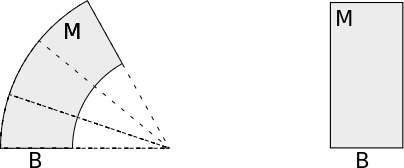
\includegraphics[width=.9\linewidth]{../img/RiemannFibration.png}
\caption{The trivialising map is only a diffeomorphism and not an isometry \label{trivalising-map}}
\end{figure}





\begin{theorem}[Hermann]
\label{thm:Hermann}
If the fibration \(\pi: M \longrightarrow B\) is
of totally geodesic fibres then the diffeomorphisms \(\hat\gamma(0) \longrightarrow
\hat\gamma(1)\) are in fact isometries between fibres and \(M\) is then locally a
Riemannian product of \(B\) and the fibre, now equipped with its unique
metric induced by \(M\).
\end{theorem}

\begin{proof}
We need to prove that the metric on fibres \(\hat g_{(b,f)}\) does not depend on the point
\(f\) of the fibre, i.e. for every basic vector field \(X\), one has \(\mathcal{L}_X\hat g=0\), where by \(\hat g\), we mean the (0,2) symmetric tensor \((Y_1, Y_2)\mapsto \langle
\mathcal{V}Y_1, \mathcal{V}Y_2 \rangle\). Let \(U,V\) be vertical vector fields of \(M\) then
\begin{equation*}
\label{eq:calcul-Hermann}
\begin{split}
X(\hat g(U,V)) &= (\mathcal{L}_X \hat g)(U,V) + \hat g([X,U],V) + \hat g(U, [X,V])\\
       	       &=  \langle \nabla_X U, V \rangle - \langle \nabla_U X, V \rangle + \langle U, \nabla_X V \rangle - \langle U, \nabla_V X \rangle + (\mathcal{L}_X\hat g)(U,V)
\end{split}   
\end{equation*}
Hence \((\mathcal{L}_X \hat g)(U,V) = \langle \nabla_U X, V\rangle + \langle U, \nabla_V
X \rangle = -2 \langle \sff(U,V), X \rangle = 0\). Since the map \(\hat\gamma(0) \mapsto \hat\gamma(1)\) is in the one-parameter group of differomorphism
associate to a basic vector field \(X\), it preserves \(\hat g\).
\end{proof}

\subsubsection{Tension fields and harmonic fibrations.}
\label{sec:orgb002288}
We will now calculate the tension field of a fibration map \(\pi: M \longrightarrow B\).

\begin{proposition}[]
\label{prop:tension-fibration}
Let \(\pi: M^n \longrightarrow B^{n'}\) be a complete Riemannian fibration then
\begin{enumerate}
\item \(e(\pi) = n/2\).
\item Let \(M_b\) be a fibre of \(\pi\) and \(\iota_{M_b}: M_b \hookrightarrow M\) be
the inclusion. Then \(\tau(\pi) = -\pi_*\tau(\iota_{M_b})\) on \(M_b\).
\end{enumerate}
In particular, \(\pi\) is harmonic if and only if its fibres are minimal submanifolds of
\(M\), i.e. the inclusions \(\iota_{M_b}\) are harmonic.
\end{proposition}
\begin{proof}
\begin{enumerate}
\item is obvious. For 2), note that
\end{enumerate}
\[
\tau(\iota_{M_b}) = -\sum_{\sigma = 1}^{n'}{\rm div\ }(e_\sigma(P))e_\sigma(P)
\]
for any orthonormal frame \(e_\sigma(P)\) of normal vectors of \(M_{\pi(P)}\).
Take \(e_\sigma\) to be \(e_\sigma = {\rm grad\ } \pi^\sigma\) where \(\pi^\sigma\)
is the \(\sigma\)-th component of \(\pi\) in a normal coordinate of \(V\) around \(\pi(P)\). Note that \(e_\sigma\) are actually the horizontal lift of the basis vectors \(\tilde e_\sigma\) of the frame at \(\pi( P)\), and therefore are normal vectors of \(M_P\). 

Meanwhile, one has \(\tau(\pi) = -\Delta \pi^\sigma \tilde e_{\sigma}\) at \(\pi(P)\)
since the Christoffel symbols vanish at \(P\). Comparing the two vector fields, one has
\(\tau(\pi) = -\pi_*\tau(\iota_{M_b})\) at \(P\).
\end{proof}

\begin{exampl}
A complete Riemannian fibration \(\pi: M \longrightarrow B\) with totally geodesic fibres are harmonic.
\end{exampl}

\fi

\subsection{Composition of maps}
\label{sec:orgf741f55}

The following results come from direct computation of the second fundamental form and
tension field of composition of maps between Riemannian manifolds. Again, we use indices
\(i,j,k,\dots\) for \(M\), \(\alpha,\beta,\gamma,\dots\) for \(M'\) and \(a,b,c,\dots\) for \(M''\).

\begin{proposition}
\label{prop:composition-general}
Let \(f: M \longrightarrow M'\) and \(f': M' \longrightarrow M''\) be smooth maps of
Riemannian manifolds, then
\begin{equation}
\label{eq:sff-composition}
\beta(f'\circ f)^a_{ij} = \beta(f)_{ij}^\gamma f'^a_\gamma + \beta(f')_{\alpha\beta}^a f^\alpha_i f^\beta_j
\end{equation}
and
\begin{equation}
\label{eq:tension-field-composition}
\tau(f'\circ f)^a = \tau(f)^\gamma f'^a_\gamma + g^{ij}\beta(f')^a_{\alpha\beta} f^\alpha_i f^\beta_j 
\end{equation}
Therefore,
\begin{center}
\begin{tabular}{lll}
If \(f'\) is & and \(f\)  is & then \(f'\circ f\) is\\
\hline
totally geodesic & totally geodesic & totally geodesic\\
totally geodesic & harmonic & harmonic\\
\end{tabular}
\end{center}
and the inverse of a totally geodesic map is totally geodesic.
\end{proposition}


\begin{remark}
It is not true in general that the composition of harmonic maps are harmonic. For example,
if one composes the harmonic maps \(\mathbb{R} \longrightarrow
\mathbb{R}^2: x \mapsto (x,2x)\) and \(\mathbb{R}^2 \longrightarrow
\mathbb{R}: (x,y)\mapsto x^2 - y^2\), the result is \(\mathbb{R}\longrightarrow \mathbb{R}: x \mapsto -3x^2\),
which is not harmonic.
\end{remark}

\begin{proposition}[composition with immersion]
\label{prop:compo-immersion}
If \(f': M' \longrightarrow M''\) is a Riemannian immersion and \(f: M \longrightarrow
M'\) then 
\begin{enumerate}
\item Energy functionals: \(E(f) = E(f'\circ f)\).
\item Tension fields: \(\tau(f)\) is the projection of \(\tau(f'\circ f)\) to \(M'\).
\end{enumerate}
\end{proposition}
\begin{proof}
\begin{enumerate}
\item One has \(e(f) = \frac{1}{2}\langle g, f^* g' \rangle  = \frac{1}{2}\langle g,
   (f'\circ f)^* g'' \rangle = e(f'\circ f)\).
\item One has \(\tau(f'\circ f)^a  = \tau(f)^a +
   g^{ij}\beta(f')^a_{\alpha\beta} f^\alpha_i f^\beta_j\) by
\eqref{eq:tension-field-composition}. The conclusion follows since the second term is normal to \(M'\).
\end{enumerate}
\end{proof}

The following immediate corollary of Proposition \ref{prop:compo-immersion} is a
generalization of the fact that a curve on a surface \(M'\) of \(\mathbb{R}^3\) is geodesic of if and only if its curvature vector is
orthogonal to \(M'\).

\begin{corollary}
If \(f': M' \longrightarrow M''\) is a Riemannian immersion, then a map \(f: M \longrightarrow M'\) is harmonic if and only if \(\tau(f'\circ f) \perp M'\).
\end{corollary}


\iffalse


\begin{proposition}[composition with submersion]
\label{prop:compo-submersion}
Let \(f': M' \longrightarrow M''\) be a Riemannian fibration with totally geodesic
fibres and \(f: M \longrightarrow M'\) then 
\[
\tau(f'\circ f) = f'_*(\tau(f))  
\]
\end{proposition}

\begin{proof}
One can suppose that \(M'\) is a Riemannian product of \(M''\) and its fibre, and
\(f'\) is the projection to \(M''\), since this is true locally and the proposition is
local. Then the conclusion is that the tension field of the projection is the projection
of the tension field, or equivalently the tension field of \(f= f_1\times f_2: M \longrightarrow
M''\times F\) is \(\tau(f) = (\tau f_1,\tau f_2)\). This follows from the explicit
formula of \(\tau(f)\), noting that the Christoffel symbols \(\Gamma^\alpha_{\beta\gamma}\) vanish except when the indice \(\alpha,\beta,\gamma\)
belong to the same tangent space (\(TM''\) or \(TF\)).
\end{proof}

\begin{exampl}
\begin{enumerate}
\item A map \(f: M \longrightarrow M'\times M''\) is harmonic if \(f=(f^1, f^2)\) with \(f^1, f^2\) harmonic.
\item Take \(M''=M\) in Proposition \ref{prop:compo-submersion} and \(f=s: M \longrightarrow M'\) a
section of the fibration \(f'\), one sees that the tension field \(\tau(s)\) is
always vertical.
\end{enumerate}
\end{exampl}

The following corollary is immediate.
\begin{corollary}
\label{cor:compo-with-submersion}
Let \(f': M' \longrightarrow M''\) be a proper Riemannian embedding and \(N\) is a
normal turbular neighborhood of \(M'\) which can be seen as a smooth fiber bundle over
\(M'\). Denote by \(\pi: N \longrightarrow M'\) the projection. Then for all map \(f:
M \longrightarrow N\), \(\pi\circ f\) is harmonic if and only if \(\tau(f)\) is vertical. 
\end{corollary}

\fi



\section{Nonlinear heat flow: Global equation and existence of harmonic maps.}
\label{sec:org2302b51}
\subsection{Statement of the main results.}
\label{sec:org6c0a559}

We want to prove in the next part existence of harmonic map between manifolds \(M\)
and \(M'\) by deforming any map \(f: M
\longrightarrow M'\) using the \(\tau\)-flow, meaning solving the PDE:
\begin{equation}
\label{eq:loc-heat-flow}
\begin{cases}
\frac{d f_t}{d t} = \tau (f_t),  & t\in [\alpha,\omega] \\
f_\alpha = f, & 
\end{cases}
\end{equation}
The equation makes sense because both \(\frac{d f_t}{d t}\) and \(\tau (f_t)\) are
vector fields along \(f_t\). Since this is the gradient-descent equation for \(E\),
the energy of \(f_t\) decreases and we hope, under conditions, to obtain
convergence of \(\{f_t\}\) to a critical point \(f_\infty\) of \(E\), this will prove
that any homotopy class of \(C^\infty(M,M')\) has at least a harmonic map.

It is proved by Eells and Sampson \cite{eells_harmonic_1964} that
\begin{theorem}[Eells-Sampson]
\label{thm:eells-sampson}
Let \(M\) and \(M'\) be compact Riemannian manifolds with \({\rm Riem } (M') \leq 0\) then there exists a harmonic map \(f: M \longrightarrow M'\) in each homotopy class.
\end{theorem}

Several boundary conditions, of Dirichlet, Neumann or mixed type, are also taken into account by Hamilton
\cite{hamilton_harmonic_1975}, as an example, we will state the Dirichlet problem:

\begin{theorem}[Hamilton]
\label{thm:hamilton-bndry-Dirichlet}
Let \(M\) and \(M'\) be compact Riemannian manifolds possibly with boundary. Suppose
that \(M'\) has \({\rm Riem } (M')\leq 0\) and \(\partial M'\) is convex, then any
relative homotopy class of \(C^\infty(M,M')\) has a harmonic element. 
\end{theorem}

About the terminology, \textbf{relative homotopy class} means that we only deform \(f\) among
maps with the same value on \(\partial M\). The \textbf{convexity of \(\partial M'\)} means
that the geodesic at any point in \(\partial M'\) with initial tangent vector parallel
to the boundary does not enter the interior of \(M'\) in short time. This condition can be expressed
using  the Christoffel symbols of \(M'\) at the point in question: If \(M'\) is
coordinated by \(y^1,\dots,y^n\) with and \(M' =\{y^n\geq 0\}\), then the convexity is
translated as \(\Gamma'^n_{\alpha\beta} \geq 0\) as a symmetric form (\(1\leq\alpha,\beta \leq n-1\)). This can be seen by the geometric intepretation of the second fundamental form of the
embedding \(s: \partial M' \hookrightarrow M'\), which is \(\sff(s) = -\Gamma'^n_{\alpha\beta}\).

It is easy to see that the convexity of \(\partial M'\) is a necessary condition, as
harmonic maps from \(\mathbb{R}\) are geodesics: Suppose the condition does not hold at
\(x\in \partial M'\), meaning that upto time \(t\) the geodesic flow of \(M'\)
initially pointing into
\(M'\) remains in the interior. The geodesic of \(\partial M'\) of length
less than \(t\) with the same initial tangent therefore cannot be deformed into a
geodesic of \(M'\) in relative homotopy class. 

\subsection{Strategy of the proof.}
\label{sec:orgc9815c3}
In order to have a global frame, we will embed \(M'\) into an Euclidean space \(V\),
but we will not use the Euclidean metric of \(V\). In fact, let \(T\) be a tubular
neighborhood of \(M'\) in \(V\) then if \(T\) is trivial, i.e. if it is diffeomorphic to \(M'\times D\)
where \(D\) is a sufficiently small ball of dimension being the codimension of \(M'\) in \(V\), and we will equip \(T\) with the product metric of \(M'\times D\). 

If \(T\) is not trivial, using a partition of unity of \(M'\), one can construct a metric on \(T\)
as linear combination of the product metrics on trivialised pieces so that
the involution \(\iota: T \longrightarrow T\) locally given by \((y,d)\mapsto (y,-d)\)
for \(y\in M', d\in D\) is an isometry. As a consequence, \(M'\) is totally geodesic
in \(T\).


Since \(M' \equiv M'\times \{0\}\) is totally geodesic in \(T\), one has for every smooth
function \(f: M \longrightarrow M'\):
\[
 \tau_T(f) = \tau_{M'} (f)
\]

The crucial property we expect for a global equation of \eqref{eq:loc-heat-flow}, is the following: if
the solution initially is in \(M'\subset V\) then it remains in \(M'\) for all
relevant time \(t>\alpha\). Eells-Sampson \cite{eells_harmonic_1964} did this by using at
the same time 2 different metrics on \(T\), namely the product metric as tubular
neighborhood and the Euclidean metric. I choose to present here the formulation of
Hamilton, which is conceptually simpler with the only drawback being that we need to
establish the uniqueness of solution of \eqref{eq:loc-heat-flow} first.

After having the global equation, we will prove the short time existence of solution by
linearising the equation and using Inverse function theorem. The global formulation and the
proof of short-time existence are independent of the negative curvature hypothesis, which
will only be used later to establish energy estimates and assure the convergence of
long-time solution and the vanishing of its tension field.


\subsection{Global equation and Uniqueness of nonlinear heat equation.}
\label{sec:orge05193d}
\begin{theorem}[Global equation]
\label{thm:global-eq}
If the smooth function \(F_t:\ M\times [\alpha,\beta] \longrightarrow V\) satisfies
\begin{equation}
\label{eq:global-heat}
\frac{d F_t}{dt} = \tau_T(F_t)
\end{equation}
and \(F_t(M\times \{\alpha\}) \subset M'\) then \(F_t(M\times[\alpha,\omega])\subset M'\)
\end{theorem}
\begin{proof}
Let \(\iota\) be the isometry of \(T\) locally given by \((y,d)\mapsto (y,-d)\) for \((y,d)\in M'\times D \equiv T\) 
and pose \(G_t= \iota F_t\) then \(G_t\) and \(F_t\) coincide initially since \(M'\) is
fixed by \(\iota\). Moreover
\[
\frac{d G_t}{d t} = d\iota . \frac{d F_t}{d t} = d\iota (\tau_T(F_t)) = \tau_T(\iota F_t)=\tau_T(G_t)
\]
We conclude that \(F_t = G_t = \iota F_t\), hence \(F_t\) remains in \(M'\) for all
relevant \(t\), using the following uniqueness of nonlinear heat equation.
\end{proof}

\begin{theorem}[Uniqueness of solution of nonlinear hear equation]
\label{thm:unique-nonlinear-heat}
Let \(f_1,f_2: M\times [\alpha,\omega] \longrightarrow M'\) be \(C^2\)
functions satisfying the non-linear heat equation
\(\frac{d f_i}{d t} = \tau_{M'}(f_i)\), i.e.
\[
 \frac{d f^\gamma}{d t} =-\Delta f^\gamma +g^{ij}\Gamma'^{\gamma}_{\alpha\beta} f^{\alpha}_{i}f^{\beta}_{j}
\]
where \(\Gamma'^\gamma_{\alpha\beta}\) are Christoffel symbols of \(M'\). Suppose that
\(f_1\) and \(f_2\) coincide on \(M\times \{\alpha\}\). Then \(f_1=f_2\) on \(M\times[\alpha,\omega]\).
\end{theorem}

\begin{proof}
It is sufficient to prove the theorem for \(\omega\) very close to \(\alpha\),
therefore by compactness of \(M\), we can suppose that there exists a finite atlas \(M
= \bigcup_i U_i\) with \(f_1 (U_i\times [\alpha,\omega])\) and \(f_2
(U_i,[\alpha,\omega])\) being in the same chart \(V_i\) of \(M'\). We consider the
distance function \(\sigma(a,b) = \frac{1}{2}d_{M'}(a,b)^2\) for \(a,b\in M'\) to
measure the difference between \(f_1\) and \(f_2\) by 
\[
 \rho(x,t) = \sigma(f_1(x,t), f_2(x,t))
\]
The strategy is to prove that there exists \(C>0\) such that \(\frac{d \rho}{d t} \leq
-\Delta \rho + C\rho\), then by \href{elliptic-parabolic.org}{Maximum principle}, one has \(\rho = 0\).

Fix a chart \(U_i\) of \(M\) and the corresponding \(V_i\) of \(M'\), one has by
straightforward calculation:
\begin{align}
 \frac{d\rho}{d t} &= -\Delta \rho -g^{ij}\left( \frac{\partial^2 \sigma}{\partial
 f_1^\beta \partial f_1^\gamma} - \frac{\partial \sigma}{\partial f_1^\alpha} {\Gamma'}
^{\alpha}_{\beta\gamma}(f_1) \right) {f_1}^\beta_i {f_1}^\gamma_j \nonumber \\
	        &- g^{ij}\left( \frac{\partial^2 \sigma}{\partial
 f_2^\beta \partial f_2^\gamma} - \frac{\partial \sigma}{\partial f_2^\alpha} {\Gamma'}
^{\alpha}_{\beta\gamma}(f_2) \right) {f_2}^\beta_i {f_2}^\gamma_j - 2g^{ij}\frac{\partial^2 \sigma}{\partial f_1^\beta \partial f_2^\gamma} {f_1}^\beta_i {f_2}^\gamma_j  \label{eq:drho-dt}
\end{align}
where \(g^{ij}\) is the metric on \(M\) and \({\Gamma'}^\alpha_{\beta\gamma}\) are
Christoffel symbols of \(M'\). 


Let \(c\) be a point in the chart \(V_i\) and choose the normal coordinates of \(M'\) at \(c\). Then for \(a,b\in M'\) near \(c\), one has, since \(\sigma(a,b) =
\sigma(b,a)\) and \(\sigma(a,b)=0\) if \(b^\gamma = k a^\gamma\) (the Euclidean
straight line from \(a\) to \(ka\) viewed on \(M'\) is a geodesic):
\[
 \sigma(a,b) = \frac{1}{2}d_{M'}(a,b)^2 = \frac{1}{2}d_E(a,b)^2 +
\lambda_{\beta\gamma,\delta}(a^\beta a^\gamma b^\delta + b^\beta b^\gamma a^\delta)
\]
where \(d_E\) is the Euclidean distance, with \(\lambda_{\beta\gamma,\delta} =
\lambda_{\gamma\beta,\delta}\) and \(\lambda_{\beta\gamma,\delta}
+\lambda_{\gamma\delta,\beta} + \lambda_{\beta\delta,\gamma}= 0\). We then have the
series development of \(\sigma\) at \((0,0)\):
\begin{equation}
\label{eq:dev-sig-unique}
\sigma(a,b) = \frac{1}{2}\delta_{\beta\gamma} (a^\beta - b^\beta)(a^\gamma - b^\gamma) +
\lambda_{\beta\gamma,\delta} (a^\beta a^\gamma b^\delta + b^\beta b^\gamma a^\delta) + O(|a|+|b|)^4
\end{equation}
and the development of its derivatives
\begin{align*}
  \frac{\partial^2 \sigma}{\partial a^\beta \partial b^\gamma}(a,b) &= -\delta_{\beta\gamma} + O(|a|+|b|)^2\\
  \frac{\partial^2 \sigma}{\partial a^\beta \partial a^\gamma}(a,b) &= \delta_{\beta\gamma} + \lambda_{\beta\gamma,\delta}b^\delta + O(|a|+|b|)^2\\
  \frac{\partial^2 \sigma}{\partial b^\beta \partial b^\gamma}(a,b) &= \delta_{\beta\gamma} + \lambda_{\beta\gamma,\delta}a^\delta + O(|a|+|b|)^2\\
   \frac{\partial\sigma}{\partial a^\alpha}(a,b) &= O(|a|+|b|),\quad {\Gamma'}^\alpha_{\beta\gamma}(a) = O(|a|)
\end{align*}
So choose \(c\) to be the midpoint of \(f_1(x,t)\) and \(f_2(x,t)\) and \((f_1(x,t),
f_2(x,t)) = (w,-w)\) in the chart, one has:
\begin{align}
 \frac{d\rho}{d t} &= -\Delta\rho - \left( \delta_{\beta\gamma} -\lambda_{\beta\gamma,\delta}w^\delta + O(|w|^2)  \right) {f_1}^\beta_i {f_1}^\gamma_j g^{ij}   - \left( \delta_{\beta\gamma} + \lambda_{\beta\gamma,\delta} w^\delta + O(|w|^2)\right) {f_2}^\beta_i {f_2}^\gamma_j g^{ij}  \label{eq:sym-red-beta-before}\\
		   & - 2\left( -\delta_{\beta\gamma} + O(|w|^2)  \right) {f_1}^\beta_i {f_2}^\gamma_j g^{ij} \label{eq:sym-red-beta}\\
		   & = -\Delta \rho - |df_1 -df_2|^2 - w^\delta \lambda_{\beta\gamma,\delta}g^{ij}\left(  {f_2}^\beta_i {f_2}^\gamma_j - {f_1}^\beta_i {f_1}^\gamma_j  \right) + O(|\omega|^2) \label{eq:first-order-w}
\end{align}
The last term of \eqref{eq:first-order-w} can be bounded as follows:
\begin{align*}
    \left | w^\delta \lambda_{\beta\gamma,\delta}\left({f_2}^\beta_i {f_2}^\gamma_j -
{f_1}^\beta_i {f_1}^\gamma_j\right) g^{ij} \right| &=   \left | w^\delta \lambda_{\beta\gamma,\delta}\left({f_2}^\beta_i ({f_2}^\gamma_j - {f_1}^\gamma_j) + {f_1}^\gamma_j({f_2}^\beta_i -
{f_1}^\beta_i) \right) g^{ij} \right| \\
	       &\leq 2 |w^\delta \lambda_{\beta\gamma,\delta}| |df_2 -df_1| (|df_1| + |df_2|)\\
	       &\leq |df_1 - df_2|^2 + O(|w|^2)
\end{align*}
where for the last inequality, we use \(2uv \leq u^2 + v^2\) and the fact that \(|df_1|\) and \(|df_2|\) are bounded on \(M\). The estimate \eqref{eq:first-order-w} can be
continued:
\[
 \frac{d \rho}{d t}\leq -\Delta\rho + C(x,t) |w|^2 \leq -\Delta \rho + C \rho
\]
where \(C >0\) is a constant chosen to dominate all \(C(x,t)\) for \(x\in M\) in all
charts and \(t\in [\alpha,\omega]\).
\end{proof}

\begin{remark}
\label{rem:hamilton-alg-rig}
The original proof of \cite{hamilton_harmonic_1975}
made the reduction of the first order of \(w\) in \eqref{eq:sym-red-beta} using
the following development of \(\sigma\):
\[
 \sigma = \frac{1}{2}\delta_{\beta\gamma} (a^\beta - b^\beta)(a^\gamma - b^\gamma) +
\lambda_{\beta\gamma,\delta} (a^\beta - b^\beta)(a^\gamma -b^\gamma)(a^\delta + b^\delta) + O(|a|+|b|)^4
\]
which was justified by \(\sigma(a,b) = \sigma(b,a)\) and \(\sigma(a,a)=0\). It can be proved that this is equivalent to \eqref{eq:dev-sig-unique} and the symmetries \(\lambda_{\beta\gamma,\delta} =
\lambda_{\gamma\beta,\delta},\ \lambda_{\beta\gamma,\delta}
+\lambda_{\gamma\delta,\beta} + \lambda_{\beta\delta,\gamma}= 0\).

As a side note, if \(a,b,c\) are on \(\mathbb{S}^2\) with \(d(a,c) = d(b,c) = x \ll 1\)
and the lines from \(a\) and \(b\) to \(c\) are orthogonal at \(c\), then the
geodesic distance \(d(a,b) = \arccos(\cos^2(x)) = x\sqrt{2} - \frac{1}{6\sqrt{2}}x^3 +
O(x^4)\). So \(\sigma(a,b) = \frac{1}{2}d(a,b)^2\) has no third-order term.
\end{remark}

\section{A few energy estimates.}
\label{sec:orgddb356b}
\subsection{Estimate of density energies}
\label{sec:org56537f7}
We finish this part with a few straightforward computation concerning the \textbf{potential
energy} \(e(f_t) = \frac{1}{2}|\nabla f_t|^2\) and the \textbf{kinetic energy} \(k(f_t) =
\frac{1}{2}|\frac{d f_t}{d t}|^2\) of a nonlinear heat flow \(f_t\)
satisfying \eqref{eq:loc-heat-flow}.

\begin{theorem}[Density of Potential energy]
\label{thm:den-pot}
If \(f_t\) satisfies \eqref{eq:loc-heat-flow} then 
\[
 \frac{d e(f_t)}{dt}= -\Delta e(f_t) - |\beta(f_t)|^2 - \left\langle \Ric(M) \nabla_v
f_t,\nabla_v f_t \rangle + \langle \Riem(M') (\nabla_v f_t,\nabla_w f_t)\nabla_v
f_t,\nabla_w f_t \right\rangle
\]
where \(e(f_t)\) is the potential energy density and \(\beta(f_t)\) is the fundamental
form and in the curvature terms, the vectors \(v\) and \(w\) are contracted.

In particular, if  \(\Riem(M') \leq 0\) and \(\Ric(M)\geq -C\) then
\begin{equation}
\label{eq:den-pot-est}
\frac{d e}{dt} \leq -\Delta e + Ce - |\beta(f_t)|^2
\end{equation}
\end{theorem}
\begin{proof}
Apply Lemma \ref{lem:calculs-general} to \(s = d f_t\) and the Riemannian-connected
bundle \(F^* TM'\) over \(M\times [\alpha,\omega]\) where \(F(\cdot,t) = f_t\), the curvature terms cancel
out and it remains to see that
\(\frac{d e(f_t)}{dt}= - \langle df_t, \Delta df_t \rangle\), meaning that \(\tilde \nabla_{\partial t} df_t = -\Delta df_t\). This can be easily
justified:
\[
\tilde \nabla_{\partial t} df_t = \tilde \nabla_{\partial t} \tilde\nabla^M F=  \tilde\nabla^M
\tilde\nabla_{\partial t} F= \tilde\nabla^M\ \tau (f_t) = -D\delta (df_t) = -\Delta df_t
\]
where the last "=" is due to \(D df_t = 0\). Note that \(D\) and \(\delta\)
are the exterior derivative and its adjoint of the bundle \((f_t)^*TM'\) on \(M\),
where \(t\) can be fixed after the third "=" sign.
\end{proof}

\begin{theorem}[Density of Kinetic energy]
\label{thm:den-kin}
If \(f_t\) satisfies \eqref{eq:loc-heat-flow} then 
\[
 \frac{d k(f_t)}{dt}= -\Delta k(f_t) - \left|\nabla \frac{\partial f_t}{\partial t}\right|^2 +
\left\langle \Riem(M') (\nabla_v f_t,\frac{\partial f_t}{\partial t})\nabla_v
f_t,\frac{\partial f_t}{\partial t} \right\rangle
\]
where \(k(f_t)\) is the kinetic energy density and in the curvature terms, the vectors \(v\) is contracted,

In particular, if  \(\Riem(M') \leq 0\) then
\begin{equation}
\label{eq:den-kin-est}
\frac{d k}{dt} \leq -\Delta k  - \left|\nabla \frac{\partial f_t}{\partial t}\right|^2
\end{equation}
\end{theorem}

\begin{proof}
Let \(F:\ I\times M \longrightarrow M'\) be the total function with \(F(t,\cdot)
= f_t\) for \(t\in I =[\alpha,\omega]\) and \(E = F^* TM'\) is a Riemannian-connected bundle on \(I\times M\) with curvature form \(\Theta\), then
\begin{equation}
\label{eq:den-kin-1}
\tilde \nabla_{\partial t} \tilde\nabla_v (dF.v) = \tilde\nabla_v \tilde\nabla_{\partial t} (dF.v) + \Theta(\partial t, v) dF.v
\end{equation}
where \(dF\) is the exterior derivative of \(f_t\) on \(M\). Note that \(\tilde \nabla_v \tilde \nabla_{\partial t} (dF.v) = \tilde \nabla_v (\tilde
\nabla_{\partial t} dF).v = \tilde \nabla_v (\tilde\nabla^M \frac{\partial f_t}{\partial
t}).v\) since \(\tilde\nabla^M \frac{\partial f_t}{\partial t}= \tilde\nabla_{\partial
t}^{I\times M} dF = \tilde\nabla^{I}_{\partial_t}dF\) because
\(\tilde \nabla\) is torsionless on \(M'\). Plugging this in \eqref{eq:den-kin-1} and taking contraction
in \(v\), one has
\begin{equation}
\label{eq:den-kin-2}
 \tilde \nabla_{\partial t}\ \tau(f_t) = -\tilde \Delta \frac{\partial f_t}{\partial t} +
\tr \left( v\mapsto \Theta (\partial t,v) dF.v\right)
\end{equation}
But \(\Theta^\beta_\alpha = R'^\beta_{\alpha\nu\mu} F^\mu_i F^\nu_j dx^i\otimes dx^j\)
where \(R'\) denotes the Riemannian curvature of \(M'\) and the indices \(i,j\) can
be \(0\), with \(x^0 \equiv t\). Hence 
\[
 \Theta (\partial t, v) dF.v = R'^\beta_{\alpha \nu \mu} \frac{\partial f^\mu_t}{\partial
t}\frac{\partial f_t^\nu}{\partial v} \frac{\partial f_t^\alpha}{\partial v} \tilde
e_\beta = \Riem(M')\left(\nabla_v f_t, \frac{\partial f_t}{\partial t}\right)\nabla_v f_t
\]
Plugging in \eqref{eq:den-kin-2} and taking inner product with \(\frac{\partial
f_t}{\partial t}\), one has
\begin{align*}
 \frac{\partial k(f_t)}{\partial t} &= \left\langle \tilde \nabla_{\partial t}\ \tau(f_t),
\frac{\partial f_t}{\partial t} \right \rangle = - \left\langle \tilde \Delta \frac{\partial
f_t}{\partial t}, \frac{\partial f_t}{\partial t} \right\rangle + \left \langle \Riem(M')
(\nabla_v f_t, \frac{\partial f_t}{\partial t}) \nabla_v f_t, \frac{\partial f_t}{\partial
t} \right \rangle  \\
   &= - \Delta \left(\frac{1}{2} \left|\frac{\partial f_t}{\partial t}\right|^2\right) - \left| \tilde \nabla \frac{\partial f_t}{\partial t}\right|^2 + \left \langle \Riem(M')
(\nabla_v f_t, \frac{\partial f_t}{\partial t}) \nabla_v f_t, \frac{\partial f_t}{\partial
t} \right \rangle
\end{align*}
\end{proof}

\subsection{Estimate of total energies}
\label{sec:org6e59536}

We will now work with the total energies, in particular the \textbf{total potential energy} \(E(f_t) := \int_M e(f_t)\) and \textbf{total kinetic energy} \(K(f_t) := \int_M k(f_t)\). Since
tension field is the gradient of \(E\), one has:

\begin{theorem}
\label{thm:energy-cons}
If \(f_t: M \longrightarrow  M'\) satisfies \eqref{eq:loc-heat-flow} then
\[
 \frac{d E(f_t)}{dt} = -\int_M \left\langle \tau(f_t), \frac{\partial f_t}{\partial t}
\right \rangle = -\int_M |\tau(f_t)|^2 = -2K(f_t) \leq 0.
\]
\end{theorem}

Integrating Theorem \ref{thm:den-kin} on \(M\) then using Theorem \ref{thm:energy-cons}, one obtains:

\begin{theorem}
\label{thm:int-den-kin}
If \(f_t\) satisfies \eqref{eq:loc-heat-flow} and \(\Riem(M')\leq 0\) then \(\frac{d
}{dt}K(f_t) \leq 0\) and one has
\begin{enumerate}
\item The total potential energy \(E(f_t)\) is \(\geq 0\), decreasing and convex.
\item The total kinetic energy \(K(f_t)\) is \(\geq 0\), decreasing and if \(\omega =
   +\infty\) then \(\lim_{t\to\infty} K(f_t) = 0\).
\end{enumerate}
In particular, \(\int_{M\times \{\tau\}} |\nabla f|^2\) and \(\int_{M\times\{\tau\}} \left|
\frac{\partial f_t}{\partial t} \right|^2\) are bounded above by a constant \(C>0\)
independent of the time \(\tau \in[\alpha,\omega]\).
\end{theorem}
Note that we ruled out the case \(K(f_t)\) decreases to a strictly positive limit
because \(E(f_t)\) is bounded below and \(\frac{d }{d t} E(f_t) = -2K(f_t)\).


Integrating Theorem \ref{thm:den-pot} on \(M\) then using Theorem \ref{thm:int-den-kin}, one has:

\begin{theorem}
\label{thm:int-den-pot}
If \(f_t\) satisfies \eqref{eq:loc-heat-flow} and \(\Riem(M')\leq 0\) and \(\Ric(M)\)
is bounded below then 
\[
\int_M |\beta(f_t)|^2 \leq C
\]
for all time \(t\) where the constant \(C\) only depends on the curvature of \(M, M'\) and the initial total potential and kinetic energy, in particular, \(C\) does not depend on \(t\).
\end{theorem}

This means that \(\|f_t\|_{W^{2,2}(M)}\) is bounded by a constant \(C\) only depending
on the curvatures and initial total energies.


\begin{corollary}[Boundedness in \( W^{2,2}(M) \)]
\label{cor:bound-2-2}
If \(F_t\) satisfies \eqref{eq:global-heat} and \(\Riem(M')\leq 0\) and \(\Ric(M)\)
is bounded below then
\[
\|F_t\|^2_{W^{2,2}(M)} := \int_M | \beta(F_t)|^2 + |\nabla F_t|^2 +|F|^2 \leq C
\]
for all time \(t\) where the constant \(C\) only depends on the curvature of \(M, M'\) and the initial total potential and kinetic energy, in particular, \(C\) does not depend on \(t\).
\end{corollary}

Note that the term \(|F|^2\) is trivially bounded since the image of \(F\) remains in
an Euclidean ball \(B\).

\iffalse
\bibliographystyle{alpha}
\bibliography{../res/Stage2018}
\fi
